\documentclass[10pt,a4paper]{article}
\usepackage{graphicx}
\usepackage{biblatex}
\usepackage{parskip}
\usepackage{listings}
\usepackage{caption}
\usepackage{subcaption}
\usepackage{amsmath}
\usepackage{amssymb}
\usepackage{multicol}
\usepackage[most]{tcolorbox}

\lstset{basicstyle=\ttfamily, breaklines = true, tabsize=2}
\graphicspath{ {./Images/} }
\setlength{\parskip}{1em}
\begin{document}
%%%%%%%%%%%%%%%%%%%%%%%%%%%%%%%%%%%%%%%%%%%%%%%%%%%%%%%%%%%%%%%%%%%%%%%%%%%%%%%%%%%%%%%%%%%%%%%%%%%%%%%%%%

\begin{titlepage}
	\centering
	{\scshape\LARGE Imperial College London \par}
	\vspace{1cm}
    {\scshape\Large Discrete Mathematics: Year 2\par}
    \vspace{1.5cm}
	{\huge\bfseries Big-O and Complexity\par}
	\vspace{2cm}
	{\Large\ Xin Wang }
	\vfill
	{\large \today\par}
\end{titlepage}

%%%%%%%%%%%%%%%%%%%%%%%%%%%%%%%%%%%%%%%%%%%%%%%%%%%%%%%%%%%%%%%%%%%%%%%%%%%%%%%%%%%%%%%%%%%%%%%%%%%%%%%%%%

\begin{abstract}
    Algorithms are at the heart of computing which is a significant area in EIE. The design and
    analysis of algorithms are essential skills to an engineer and there several established design
    and analysis strategies. \par 

    Understanding "Time Complexity" is important in order to write fast code. Time Complexity is the
    computational complexity that describes the amount of time it takes to run an algorithms.
\end{abstract}

%%%%%%%%%%%%%%%%%%%%%%%%%%%%%%%%%%%%%%%%%%%%%%%%%%%%%%%%%%%%%%%%%%%%%%%%%%%%%%%%%%%%%%%%%%%%%%%%%%%%%%%%%%

\tableofcontents
\pagebreak

%%%%%%%%%%%%%%%%%%%%%%%%%%%%%%%%%%%%%%%%%%%%%%%%%%%%%%%%%%%%%%%%%%%%%%%%%%%%%%%%%%%%%%%%%%%%%%%%%%%%%%%%%%
\section{Introduction}

\begin{tcolorbox}[breakable,colback=white]
\textbf{Algorithm}: A sequence of computational steps that takes a value as \textbf{input}
and produces one/set of values as \textbf{output}.
\\
\\
\textbf{Instance} (of a problem): Consists of the input (satisfying any program constraints)
required to compute a solution to the problem.
\end{tcolorbox}

Algorithms have many practical applications in fields such as biology and com-
puting e.g. sorting algorithms which are common since any computational pro-
grams will often have sorting elements in it. The data produced by algorithms
are then stored in data structures for review or further processing.

\begin{tcolorbox}[breakable,colback=white]
\textbf{Data structures}: A way to store and organize data in order to facilitate access and
modifications. There are various types and each have their own advantages and disadvantages.
\end{tcolorbox}

Algorithms are divided into two major sections: Design and Analysis.

%%%%%%%%%%%%%%%%%%%%%%%%%%%%%%%%%%%%%%%%%%%%%%%%%%%%%%%%%%%%%%%%%%%%%%%%%%%%%%%%%%%%%%%%%%%%%%%%%%%%%%%%%%
\subsection{Analysis of algorithms}

\begin{tcolorbox}[breakable,colback=white]
\textbf{Analysis} (of algorithms): Predicting the resources that the algorithm requires such as
memory, communication bandwidth, computer hardware and, most importantly, time.
\end{tcolorbox}

The main concept concerned in algorithm analysis is complexity notation. It
is used to compute the time an algorithm takes and prove an algorithm works.

In general, the time taken grows with the size of the input thus it is common
to describe the program running time as a function of the size of its input.

\begin{tcolorbox}[breakable,colback=white]
\textbf{Running time} (of an algorithm): The number of primitive operations "steps" executed.
\end{tcolorbox}

There are two types of running time: Worse case running time and Average
case running time.

Usually, the worst case running time is used because:
\begin{itemize}
    \item It gives the upper bound on the running time for any input and it occurs
    often.
    \item The average case is the same function as the worst case.
\end{itemize}

\pagebreak

%%%%%%%%%%%%%%%%%%%%%%%%%%%%%%%%%%%%%%%%%%%%%%%%%%%%%%%%%%%%%%%%%%%%%%%%%%%%%%%%%%%%%%%%%%%%%%%%%%%%%%%%%%
\subsection{Design of algorithms}

\begin{tcolorbox}[breakable,colback=white]
\textbf{Design} (of algorithms): A mathematical process to approach problem solving.
\end{tcolorbox}

Algorithms are fundamentally a series of steps to solve a given problem. There
are numerous types of algorithm design techniques and each technique differs
in complexity with certain advantages in different scenarios.

The design techniques to be covered are:
\begin{itemize}
    \item Divide and conquer
    \item Dynamic programming
    \item Greedy algorithms
\end{itemize}

Over the course of this course, graph algorithms are covered including general
purpose graph design methods:
\begin{itemize}
    \item Breadth first
    \item Depth first
\end{itemize}

\pagebreak

%%%%%%%%%%%%%%%%%%%%%%%%%%%%%%%%%%%%%%%%%%%%%%%%%%%%%%%%%%%%%%%%%%%%%%%%%%%%%%%%%%%%%%%%%%%%%%%%%%%%%%%%%%
\section{The Fibonacci Series}

The Fibonacci series is used to show the importance of analysis and design
of algorithms. The Fibonacci series is originally used to model the growth of
rabbits e.g.$ F(1) = 1, F(2) = 1, F(3) = 3, F(4) = 5$.

Fibonacci series F(n) is defined by:
\begin{align*}
    F(n) = F(n - 1) + F(n - 2)
\end{align*}

There are several different ways to compute Fibonacci series, each with various
efficiency.

%%%%%%%%%%%%%%%%%%%%%%%%%%%%%%%%%%%%%%%%%%%%%%%%%%%%%%%%%%%%%%%%%%%%%%%%%%%%%%%%%%%%%%%%%%%%%%%%%%%%%%%%%%
\subsection{Recursion}

This algorithm is very simple but very inefficient since this algorithm repeatedly
has to compute the same values again and again i.e. F(4) computes F(3) and
F(2) in which F(3) computes F(2) and F(1) again:

\begin{lstlisting} [numbers=none]
def F_recurse (n):
    if n <=2:
        return 1
    else:
        return F_recurse (n -1) + F_recurse (n -2)
\end{lstlisting}

\begin{figure} [h!]
    \centering
    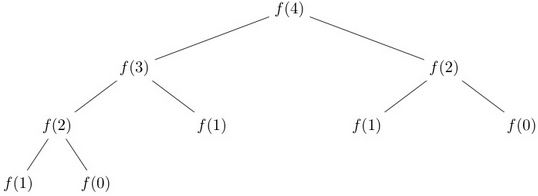
\includegraphics[scale=0.7]{Fibonacci.JPG}
    \caption{Recursion tree of Fibonacci series}
\end{figure}

Calculating any value in the Fibonacci series only requires the previous
two values e.g. F(4) only requires F(3) and F(2). So a more efficient algorithm
would store the last two values to calculate the next value in the Fibonacci
series.

\pagebreak

%%%%%%%%%%%%%%%%%%%%%%%%%%%%%%%%%%%%%%%%%%%%%%%%%%%%%%%%%%%%%%%%%%%%%%%%%%%%%%%%%%%%%%%%%%%%%%%%%%%%%%%%%%
\subsection{Pen and paper algorithm}

The two most recent values are used to calculate the next value in the Fibonacci series. This
results in higher high memory usage that increases exponentially to $n$.

\begin{lstlisting}
def F_pnp (n):
    f = [1]*( n+1) # Create the needed space
    f[1] = f[2] = 1 # Two initial values are 1

    for i in range (3, n+1):
        f[i] = f[i -1] + f[i -2]
    return f[n]
\end{lstlisting}

%%%%%%%%%%%%%%%%%%%%%%%%%%%%%%%%%%%%%%%%%%%%%%%%%%%%%%%%%%%%%%%%%%%%%%%%%%%%%%%%%%%%%%%%%%%%%%%%%%%%%%%%%%
\subsection{Iterative algorithm}

Only the two most recent values are used, only a fixed amount of RAM is used
for any n. This is the most efficient code for calculating the Fibonacci sequence.

\begin{lstlisting}
def F_iter (n):
    a = b = 1 # 1st and 2nd value of series are both 1

    for i in range (3,n+1): # Starting from 3rd
        a,b = b, a+b # Two most recent values
    return b
\end{lstlisting}

%%%%%%%%%%%%%%%%%%%%%%%%%%%%%%%%%%%%%%%%%%%%%%%%%%%%%%%%%%%%%%%%%%%%%%%%%%%%%%%%%%%%%%%%%%%%%%%%%%%%%%%%%%
\subsection{Binet’s formula}

\begin{align*}
    F(n) = \frac{\phi^n-(1-\phi)^n}{\sqrt{5}} \; \text{ where } \phi = \frac{1+\sqrt{5}}{2}
\end{align*}
With the general formula, time complexity becomes $\Theta(1)$ i.e. constant but
memory complexity is not $\Theta(1)$. This is because for each larger $n$, higher
precision would be required to represent the Fibonacci numbers.

%%%%%%%%%%%%%%%%%%%%%%%%%%%%%%%%%%%%%%%%%%%%%%%%%%%%%%%%%%%%%%%%%%%%%%%%%%%%%%%%%%%%%%%%%%%%%%%%%%%%%%%%%%
\subsection{Matrix algorithm}

Theoretically, the matrix method is the best solution:
\begin{align*}
    \begin{bmatrix}
        1&1\\1&0
    \end{bmatrix}^n = 
    \begin{bmatrix}
        F(n+1)&F(n)\\F(n)&F(n-1)
    \end{bmatrix} 
\end{align*}

This is due to a special characteristic of matrix multiplication. For example
$M^8$ would not actually need to multiply $8$ times, instead $3$ times would be
enough:
\begin{align*}
    M^8 = ((M^2)^2)^2
\end{align*}

This method results in a time complexity of $\Theta(\log(n))$ and a memory complexity
of $\Theta(1)$. But, in practice, it is not more efficient than the iterative method.


\pagebreak

%%%%%%%%%%%%%%%%%%%%%%%%%%%%%%%%%%%%%%%%%%%%%%%%%%%%%%%%%%%%%%%%%%%%%%%%%%%%%%%%%%%%%%%%%%%%%%%%%%%%%%%%%%
\section{Growth of function}%%%%%%%%%%%%%%%%%%%%%%%%%%%%%%%%%%%%%%%%%%%%%%%%%%%%%%%%%%%%%%%%%%%%%%%%%%%%%%%%%%%%%%%%%%%%%%%%%%%%%%%%%%
\subsection{Asymptotic notation}

Asymptotic notation are mathematical tools to represent the time complexity
of algorithms for asymptotic analysis when the input tends towards a particular
value or a limiting value.

Performance analysis is important since that it affects other critical aspects
such as the user experience and program modularity. When studying two given
algorithms, one might be more efficient for certain input ranges and not as
efficient for other input ranges. Asymptotic analysis shows these characteristics
by evaluating the performance of an algorithm \textbf{in terms of varying input size}.

\begin{tcolorbox}[breakable,colback=white]
    \textbf{Asymptotic analysis} (of an algorithm): Evaluates how much resources
    i.e. time or memory space is occupied by an algorithm in terms of input
    size and not the actual running time.
\end{tcolorbox}

Asymptotic notations are defined in terms of functions, including algorithms
and programs, whose domain is the set of natural numbers $$\mathbb{N} = {0,1,2,\dots}$$

It is important to realise that asymptotic notation can be applied, not only to
running time of a algorithm, but also to functions that characterise other aspects
of algorithms such as memory usage. Therefore, it is critical to understand which
aspect the asymptotic notation is applied to. Usually, asymptotic notations try
to universally characterise running time no matter the type of input - a blanket
statement that covers all inputs including worst case running times.

\begin{figure} [h!]
    \centering
    \includegraphics[scale=0.7]{little omega.JPG}
    \caption{Areas of coverage of the different domains of notations}
\end{figure}

\pagebreak

%%%%%%%%%%%%%%%%%%%%%%%%%%%%%%%%%%%%%%%%%%%%%%%%%%%%%%%%%%%%%%%%%%%%%%%%%%%%%%%%%%%%%%%%%%%%%%%%%%%%%%%%%%
\subsubsection{Theta $(\Theta)$ notation}

Theta notation is \textbf{asymptotically tight bound}, it means the function lies in
the upper and the lower bound. Graphically, it encloses the function from above
and below. It is commonly used for analysing the average case complexity of an
algorithm by using the worst-case time and best-case time.

\begin{tcolorbox}[breakable,colback=white]
For a given function $f(n)$, a function is considered equal to $\Theta(g(n))$ if
there are positive constants $c_1$, $c_2$ and $n_0$ such that:
\begin{align*}
    0 \leq c_1 * g(n) \leq f(n) \leq c_2 * g(n) \; \text{where}: n \geq n_0
\end{align*}
\end{tcolorbox}

In words, function $f(n)$ is considered to belong to the set $\Theta(g(n))$ if there
are positively defined constants $c_1$ and $c_2$ , such that from the point of value
$n_0$ towards the right, the function $f(n)$ is ”sandwiched” between $c_1* g(n)$ and
$c_2 * g(n)$ for a sufficiently large range $n$. In other words, $f(n)$ is approximately
proportional to $g(n)$.

\begin{tcolorbox}[breakable,colback=white]
    Alternatively, $\Theta$-notation can be defined as:
    \begin{align*}
        0 < c_1 \leq \frac{f(n)}{g(n)} \leq c_2
    \end{align*}
\end{tcolorbox}

A simple way to get the $\Theta$-notation of an expression is to drop low order terms
and ignore leading constants. The reason it is possible is because, remember,
asymptotic complexity is not concerned with comparing performance of different algorithms. It is for
understanding how performance of individual algorithms scales with respect to the input size.

In summary:
\begin{itemize}
    \item Ignore constant factors e.g. 3 in $3n^2$ and Theta notation is $\Theta(n^2)$
    \item Only note the asymptotic behavior i.e. $100n + 0.1n^2$ is $\Theta(n^2)$ since for
    large enough $n$ the size of the equation will be dominated by $0.1n^2$
\end{itemize}

\begin{figure} [h!]
    \centering
    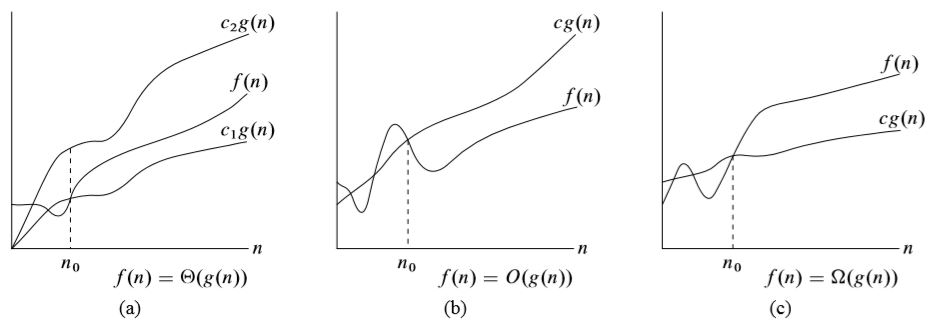
\includegraphics[scale=0.5]{Theta-notation.JPG}
    \caption{Graphical examples of $\Theta$-notation, $O$-notation and $\Omega$-notation respectively.}
\end{figure}

\pagebreak

The Theta notation $\Theta(g(n))$ is mathematically treated as a set so it is
correct to say $f(n)$ is a member of $\Theta(g(n))$ [$f(n) \in \Theta(g(n))$] where $g(n)$
are functions. However, usually it is written $f(n)=\Theta(g(n))$ which has certain advantages but
should be very carefully used. 

\begin{tcolorbox}[breakable,colback=white]
\textbf{Asymptotically tight bound}: For all values of $n$ at and to the right of $n_0$, value of
$f(n)$ lies at or above $c_1g(n)$ and at or below $c_2g(n)$. In other words, for all $n\geq n_0$,
the function of $f(n)$ is equal to $g(n)$ to within a constant factor.
\\
\\
\textbf{Asymptotically nonnegative}: $f(n)$ is nonnegative whenever $n$ is sufficiently large.
\\
\\
\textbf{Tight upper bound}: An upper bound where there are no smaller value that is a better upper
bound. 
\\
\\
\textbf{Tight lower bound}: A lower bound is the greatest lower bound, or an infimum, if no greater
value is a better lower bound. 
\end{tcolorbox}

The definition of $\Theta$-notation requires that every member of $f(n) \in \Theta(g(n))$ be
asymptotically nonnegative. Among all the notations, $\Theta$ notation gives the best intuition
about the rate of growth of function because it gives a tight bound unlike big-O and $\Omega$ which
gives the upper and lower bounds respectively. \par 

\begin{center}
    \textbf{$f(n)$ is $\Theta(g(n))$ if and only if it is $O(g(n))$ and $\Omega(g(n))$}
\end{center}

\textbf{Example 1}: Proof $f(x) = n^2 - n = \Theta(n^2)$:
\begin{itemize}
    \item List $g(n)$:
    \begin{align*}
        g(n) = n^2 \; \text{ and } \; f(n) = n^2 - n
    \end{align*} 

    \item Express as $\frac{f(n)}{g(n)}$:
    \begin{align*}
        \frac{f(n)}{g(n)} = \frac{n^2 - n}{n^2} = 1 - \frac{1}{n}
    \end{align*}

    \item Try $n_0 = 2$:
    \begin{align*}
        0 < c_1 = \frac{1}{2} \leq 1 - \frac{1}{n} \leq 1 = c_2
    \end{align*}
\end{itemize}

\pagebreak

%%%%%%%%%%%%%%%%%%%%%%%%%%%%%%%%%%%%%%%%%%%%%%%%%%%%%%%%%%%%%%%%%%%%%%%%%%%%%%%%%%%%%%%%%%%%%%%%%%%%%%%%%%
\subsubsection{Big-O ($O$) notation}

The Big-O notation is used when only the asymptotic upper bound is concerned. The Big-O gives an
upper bound on a function to within a constant factor - for all values $n$ at and to the right of
$n_0$, the function is \textbf{on or below} $c*g(n)$.

\begin{tcolorbox}[breakable,colback=white]
For a given function $f(n)$, a function is $O(g(n))$ if there are positive constants $c_0$ and $n_0$ such that:
$$
0 \leq f(n) \leq c*g(n) \; \text{ where: $n\geq n_0$}
$$
or
\begin{align*}
    0 \leq \frac{f(n)}{g(n)} \leq c \; \text{ where: $n\geq n_0$}
\end{align*}
Meaning: "Program takes at most g(n) steps to run"
\end{tcolorbox}

Like $\Theta$-notation, $f(n)=O(g(n))$ indicates that a function $f(n)$ is a member of the set
$O(g(n))$. \textbf{$f(n)=\Theta(g(n))$ implies $f(n)=O(g(n))$ since $\Theta$-notation is a stronger
notion that $O$-notation}. \par 
 
\textbf{Example 1}: $n = O(n^2)$
\begin{figure} [h!]
    \centering
    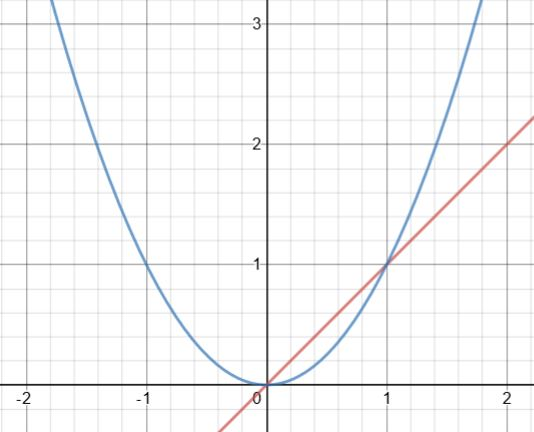
\includegraphics[scale=0.4]{Omega graph.JPG}
\end{figure}

\textbf{Example 2}: $\text { Given } f(n)=\left\{\begin{array}{ll}
    0 & n \text { even } \\
    n & n \text { odd }
    \end{array},\right. \text {prove } f(n)=O(g(n))$
\begin{itemize}
    \item List $g(n)$: $g(n)=n$
    \item Express as $\frac{f(n)}{g(n)}$:
    \begin{align*}
        \frac{f(n)}{g(n)}=\left\{\begin{array}{ll}
            0 & n \text { even } \\
            1 & n \text { odd }
            \end{array}\right.
    \end{align*}
    \item State the bounds:
    \begin{align*}
        0 \leq \frac{f(n)}{g(n)} \leq 1=c
    \end{align*}
\end{itemize}

\pagebreak

%%%%%%%%%%%%%%%%%%%%%%%%%%%%%%%%%%%%%%%%%%%%%%%%%%%%%%%%%%%%%%%%%%%%%%%%%%%%%%%%%%%%%%%%%%%%%%%%%%%%%%%%%%
\subsubsection{Big-Omega $(\Omega)$ notation}

The Big-Omega notation is used when there is only an \textbf{asymptotic lower bound}. The Big-Omega gives a
lower bound on a function to within a constant factor - for all values $n$ at and to the right of
$n_0$, the function is \textbf{on or above} $cg(n)$.

\begin{tcolorbox}[breakable,colback=white]
    For a given function $f(n)$, a function is $\Omega(g(n))$ if there are positive constants $c_0$ and $n_0$ such that:
    $$
    0 \leq cg(n) \leq f(n) 
    $$
    where: $n\geq n_0$
\end{tcolorbox}

\textbf{$f(n)=\Theta(g(n))$ implies $f(n)=\Omega(g(n))$ since $\Theta$-notation is a stronger notion that $\Omega$-notation}.

%%%%%%%%%%%%%%%%%%%%%%%%%%%%%%%%%%%%%%%%%%%%%%%%%%%%%%%%%%%%%%%%%%%%%%%%%%%%%%%%%%%%%%%%%%%%%%%%%%%%%%%%%%
\subsubsection{Little-o $o$ notation}

The asymptotic upper bound provided by $O$-notation may/may not be \textbf{asymptotically tight}
i.e. $2n^2 = O(n^2)$ is asymptotically tight but not $2n = O(n^2)$ since there will be some leeway
(Refer to Figure 2).

\begin{tcolorbox}[breakable,colback=white]
\textbf{Asymptotically tight}: A bound has the the tightest possible bounds, meaning it satisfies
the conditions of $\Theta$-notation where it requires the tightest bounds.
\end{tcolorbox}

\begin{figure} [h!]
    \centering
    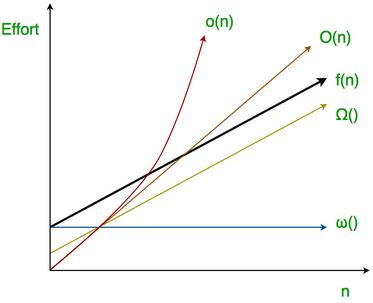
\includegraphics[scale=0.7]{Asymptotically tight.JPG}
    \caption{A graphical representation of the relationships of the four notations to $f(n)$}
\end{figure}

\begin{tcolorbox}[breakable,colback=white]
    For a given function $f(n)$, a function is $o(g(n))$ if for any constant $c>0$ there is an $n_0$
    such that:
    $$
        0 \leq f(n) < cg(n)
    $$
    where: $n\geq n_0$
\end{tcolorbox}

The main difference between Big-O and Little-O is that:
\begin{itemize}
    \item Bound $0\leq f(n) \leq cg(n)$ holds for \textbf{some} constant $c>0$
    \item Bound $0\leq f(n) < cg(n)$ holds for \textbf{all} constant $c>0$ 
\end{itemize}

Due to the definition of the little-o notation, the function $f(n)$ becomes insignificant relative
to $g(n)$ as $n$ approaches infinity.
$$
\lim_{n\rightarrow \infty} \frac{f(n)}{g(n)} = 0
$$

%%%%%%%%%%%%%%%%%%%%%%%%%%%%%%%%%%%%%%%%%%%%%%%%%%%%%%%%%%%%%%%%%%%%%%%%%%%%%%%%%%%%%%%%%%%%%%%%%%%%%%%%%%
\subsubsection{Little-omega $\omega$ notation}

The asymptotic low bound provided by $\Omega$-notation may/may not be \textbf{asymptotically tight}.

\begin{tcolorbox}[breakable,colback=white]
    For a given function $f(n)$, a function is $\omega(g(n))$ if for any positive constant $c>0$ there is an $n_0$
    such that:
    $$
        0 \leq cg(n) < f(n)
    $$
    where: $n\geq n_0$
\end{tcolorbox}

The main difference between Big-O and Little-O is that:
\begin{itemize}
    \item Bound $0\leq f(n) \leq cg(n)$ holds for \textbf{some} constant $c>0$
    \item Bound $0\leq f(n) < cg(n)$ holds for \textbf{all} constant $c>0$ 
\end{itemize}

Due to the definition of the little-o notation, the function $f(n)$ becomes insignificant relative
to $g(n)$ as $n$ approaches infinity.
$$
\lim_{n\rightarrow \infty} \frac{f(n)}{g(n)} = \infty
$$

%%%%%%%%%%%%%%%%%%%%%%%%%%%%%%%%%%%%%%%%%%%%%%%%%%%%%%%%%%%%%%%%%%%%%%%%%%%%%%%%%%%%%%%%%%%%%%%%%%%%%%%%%%
\subsection{Common Big-O Examples}
Time complexity scale:
$$
    constants < logarithms < polynomials < exponentials
$$

\textbf{Example 1}: $O(1)$

Time complexity is 1 - always just one operation. It is \textbf{constant}. $O(1)$ is the best possible time complexity as it
means constant time operations. \par 

Common example: A program removing one letter from a list.
\begin{align*}
    [a,b,c,d,e] \rightarrow [a,b,c,d]
\end{align*}

\textbf{Example 2}: $O(n)$

\textbf{Linear} - runtime is \textit{Order n} since number of operations required is
\textbf{proportional} to $n$ to be computed. The complexity of the operation does not change,
runtime is solely dependent on the size of $n$. \par 

Common example: A program that duplicates each letter in a list.
\begin{align*}
    [a,b,c,d,e] \rightarrow [aa,bb,cc,dd,ee]    
\end{align*}

\textbf{Example 3}: $O(n^c)$ where $c$ is a constant 

\textbf{Polynomial} time complexity. Usually not acceptable measure - the number of operations
required is $n^c$. $n^2$ is called quadratic time complexity e.g. a list with 3 variables will
require 9 operations. \par

Common example: A program to add every member of list to each other.
\begin{align*}
    [a,b,c,d,e] \rightarrow [abcde,bacde,cabde,dabce,eabcd]
\end{align*}

\textbf{Example 4}: $O(c^n)$ where $c$ is a constant

\textbf{Exponential} time complexity. The worse possible complexity. \par 

Common example: Brute forcing a password by trying every possible combination.

\textbf{Example 4}: $O(log(n))$

\textbf{Logarithmic} time complexity - the opposite of exponential time complexity. As the size of
$n$ increases, the smaller proportion the number of operations will be required. \par 

Common example: Looking people up in a phone book - not every person needs to be checked, able to
use divide-and-conquer to narrow the search alphabetically.

%%%%%%%%%%%%%%%%%%%%%%%%%%%%%%%%%%%%%%%%%%%%%%%%%%%%%%%%%%%%%%%%%%%%%%%%%%%%%%%%%%%%%%%%%%%%%%%%%%%%%%%%%%
\section{Divide-and-Conquer}

Divide-and-Conquer is a strategy for designing algorithms by solving a problem recursively -
applying three steps at each level of recursion.

\begin{enumerate}
    \item \textbf{Divide}: Divide problem into a number of sub-problems (smaller instances of the
    same problem).
    \item \textbf{Conquer}: Solve sub-problems by solving recursively.
    \item \textbf{Combine}: Combine solutions to the sub-problems into the solutions for the
    original problem.
\end{enumerate}

\begin{tcolorbox}[breakable,colback=white]
\textbf{Recursive case}: Sub-problems that are large enough to solve recursively.
\\
\\
\textbf{Base case}: Sub-problems that are small enough that cannot be used with recursion anymore.
\end{tcolorbox}

Sometimes dividing a problem into sub-problems can save time. 

\textbf{Example 1}: Given an algorithm defined by $O(n^2)$ where $n=128$ compare.
\begin{itemize}
    \item Normal head on approach: $n=128$ so will take $128^2 = \underline{16 384}$ steps.
    \item Divided into two: 
    \begin{itemize}
        \item $n=64$ so will take $64^2=4 096$ steps for each half.
        \item $8 192$ for each half. $128$ steps to combine solutions.
        \item Total steps required: \underline{$8 320$} 
    \end{itemize}  
\end{itemize}

%%%%%%%%%%%%%%%%%%%%%%%%%%%%%%%%%%%%%%%%%%%%%%%%%%%%%%%%%%%%%%%%%%%%%%%%%%%%%%%%%%%%%%%%%%%%%%%%%%%%%%%%%%
\subsection{Recurrence}

\begin{tcolorbox}[breakable,colback=white]
\textbf{Recurrence}: An equation/inequality that describes a function in terms of its value on
smaller inputs. 
\end{tcolorbox}

Recurrences are closely connected with the Divide-and-Conquer paradigm since it is a natural way to
characterize the running times of Divide-and-Conquer algorithms. \par 

Following \textbf{Example 1}: The recurrence can be found by finding the gain for a general $n$.
\begin{itemize}
    \item 0 divide: $n^2$
    \item 1 divide: $2\left(\frac{n}{2}\right)^2 + n = \frac{n^2}{2}+n$
    \item 2 divide: $4\left(\frac{n}{4}\right)^2 + n + 2\left(\frac{n}{2}\right)=\frac{n^2}{4}+2n$
    \par 
    \dots
    \item General divide: $2^k\left(\frac{n}{2^k}\right)^2 + n + \dots + 2^k\left(\frac{n}{2^k}\right)=\frac{n^2}{2^k}+nk$
\end{itemize}
Taking the max where $\frac{n}{2^k}=1$ thus $k=log_2n$: the recurrence is:
$$
    T(n)=O(n\text{ }log_2n)
$$

\begin{figure} [h!]
    \centering
    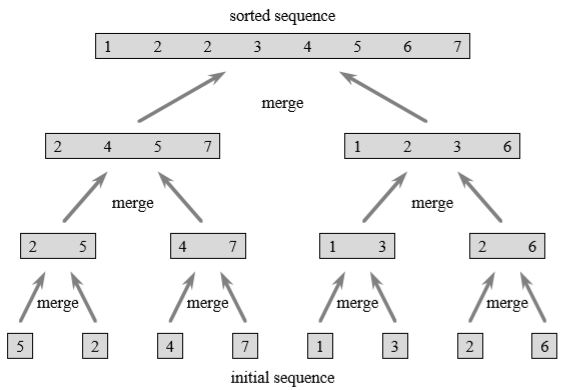
\includegraphics[scale=0.7]{DAC.JPG}
    \caption{}
\end{figure}

Recurrences can take many forms and some divide sub-problems into unequal sizes. Sub-problems are
not constrained to being a constant fraction of the original problem. There are three methods for
solving recurrences (obtaining the asymptotic $O$ bounds of the solution):
\begin{itemize}
    \item \textbf{Substitution method}: Guess a bound then use mathematical induction to prove the
    guess was correct.
    \item \textbf{Recursion-tree method}: Convert recurrence into tree whose nodes represent costs
    incurred at that level of recursion. Techniques for bounding summations are used to solve recurrence.
    \item \textbf{Master method}: Provide bounds in the form: $T(n)=aT\left(\frac{n}{b}\right)+f(n)$
    where $a \geq 1$, $b>1$ and $f(n)$ is a given function.
\end{itemize} 

%%%%%%%%%%%%%%%%%%%%%%%%%%%%%%%%%%%%%%%%%%%%%%%%%%%%%%%%%%%%%%%%%%%%%%%%%%%%%%%%%%%%%%%%%%%%%%%%%%%%%%%%%%
\subsubsection{Master method}

The master method provides a general "cookbook" approach to solving recurrences in the form:
$$
    T(n)=aT\left(\frac{n}{b}\right)+f(n)
$$
or 
$$
    T(n)=aT\left(\frac{n}{b}\right)+O(n^d)
$$
where $a\geq 1$, $b>1$ and $d\geq 0$ are constants with $f(n)$ begin an asymptotically positive function. \par 

The equation describes several points on the running time of an algorithm:
\begin{itemize}
    \item A problem of size $n$ divided into $a$ sub-problems, each of size $\frac{n}{b}$ where $a$ and $b$ are positive constants.
    \item $a$ sub-problems are solved recursively, each with time $T\left(\frac{n}{b}\right)$.
    \item Function $f(n)$ encompasses the cost of dividing the problem and combining the results of
    the sub-problems.
\end{itemize}

The Master Method is based on the \textbf{Master Theorem} which has three cases, each with its own
conditions.

\begin{equation*}
    T(n) = 
    \begin{cases}
        O(n^d) & \text{ if } d>log_b a \\
        O(n^dlog[n]) & \text{ if } d=log_ba \\
        O(n^{log_ba}) & \text{ if } d<log_ba
    \end{cases}
\end{equation*}

\textbf{Example 1}: Consider $T(n)=9T\left(\frac{n}{3}\right)+n$. \par 
\begin{enumerate}
    \item Note $a=9$, $b=3$ and $f(n)=n$ ($d=1$).
    \item Finding $log_ba$ which is $2$, it meets Case 3.
    \item $T(n)=O(n^{log_ba})=O(n^2)$
\end{enumerate}

\textbf{Example 2}: Consider $T(n)=T\left(\frac{2n}{3}\right)+1$. \par 
\begin{enumerate}
    \item Note $a=1$, $b=\frac{3}{2}$ and $f(n)=1$ ($d=0$).
    \item Finding $log_ba$ which is $0$, it meets Case 2.
    \item $T(n)=O(n^dlog[n])=O(log[n])$
\end{enumerate}

\pagebreak

%%%%%%%%%%%%%%%%%%%%%%%%%%%%%%%%%%%%%%%%%%%%%%%%%%%%%%%%%%%%%%%%%%%%%%%%%%%%%%%%%%%%%%%%%%%%%%%%%%%%%%%%%%
\section{Dynamic Programming}

Dynamic Programming applies when sub-problems \textbf{overlap} and solves the common sub-problems
just once and saves it in a table, avoiding recomputing it. The "programming" refers to tabular
programming and has nothing to do with computer programming. \par 

Dynamic Programming usually applies to \textbf{optimization problems} - where problems have many
possible solutions e.g. Google Maps to find the shortest
path between sources. Each solution has a value and the goal is to find a solution with optimal (min
or max) value. Solutions are called \textit{an optimal solution to the problem} instead of
\textit{the optimal solution to the problem} as there may be several solutions. \par 

There are two key attributes that a problem must have in order to be able to
apply dynamic programming to it:
\begin{itemize}
    \item \textbf{Optimal substructure}: An optimal solution to a problem contains optimal solutions to subproblems.
    
    Optimal solutions to whole problem $=$ combination of optimal solutions to sub-problems.
    \item \textbf{Overlapping subproblems}: A recursive solution contains a “small”
    number of distinct subproblems repeated many times.
\end{itemize}

There are four steps to developing a dynamic-programming algorithm:
\begin{enumerate}
    \item \textbf{Characterize} the structure of an optimal solution
    \item \textbf{Recursively} define the value of an optimal solution
    \item \textbf{Compute} value of an optimal solution (Usually bottom-up fashion)
    \item \textbf{Construct} an optimal solution from computed information
\end{enumerate}

There are similarities and differences between DP and DAC:
\begin{itemize}
    \item Similarities: Both partition a problem into smaller subproblems and build the solution of larger problems from solutions of smaller problems
    \item Difference:
    \begin{itemize}
        \item DAC work top-down i.e. know exact smaller problems that need to be solved to solve larger problem.
        \item DP usually work bottom-up. Solve all smaller size problems and build larger problem solutions from them.
    \end{itemize}
\end{itemize}

\pagebreak

%%%%%%%%%%%%%%%%%%%%%%%%%%%%%%%%%%%%%%%%%%%%%%%%%%%%%%%%%%%%%%%%%%%%%%%%%%%%%%%%%%%%%%%%%%%%%%%%%%%%%%%%%%
\subsection{Applying Dynamic Programming}

Mentioned earlier, a naive recursive solution is inefficient since it solves the same sub-problems
repeatedly. It would be much more efficient to solve each problem only \textbf{once} and save the
solution in memory. Dynamic programming uses additional memory to save computation time - an example
of \textbf{time-memory trade-off}. 

\begin{tcolorbox}[breakable,colback=white]
\textbf{Memoisation} - A common optimization technique used to primarily speed up computer programs by
storing results of computations and returning the cached results when same inputs occur again.
\end{tcolorbox}

There are two common ways to implement a dynamic-programming approach: \textbf{top-down with
memoization method} and \textbf{bottom-up method}. Both method are \textbf{$O(n^2)$} but bottom-up method is
more efficient.

%%%%%%%%%%%%%%%%%%%%%%%%%%%%%%%%%%%%%%%%%%%%%%%%%%%%%%%%%%%%%%%%%%%%%%%%%%%%%%%%%%%%%%%%%%%%%%%%%%%%%%%%%%
\subsubsection{Data strutures}

Types of data structures used are important in the overall efficiency of the algorithm. For example,
using array will require arguments to be integers only but often arguments are unknown. A common
solution is to use a \textbf{hash table} where a data structure $T$ maps to values $T[k]$. The
performance is slightly worse than array but advantages are many i.e. insertion/lookup/deletion are
$O(1)$ typically and $O(n)$ worse-case. \par 

\begin{tcolorbox}[breakable,colback=white]
\textbf{Optimal substructure}: If an optimal solution can be constructed from optimal solutions of
its sub-problems. Indicates the usefulness of the dynamic programming and greedy algorithms for a problem.
\end{tcolorbox}

Data structures will be covered in depth in another chapter. 

\pagebreak

%%%%%%%%%%%%%%%%%%%%%%%%%%%%%%%%%%%%%%%%%%%%%%%%%%%%%%%%%%%%%%%%%%%%%%%%%%%%%%%%%%%%%%%%%%%%%%%%%%%%%%%%%%
\subsection{Fibonacci numbers and dynamic programming}

The mathematical equation describing it is:
\begin{align*}
    F(n + 2) = F(n + 1) + Fn
\end{align*}

Solving the problem using dynamic programming, there are two approaches in Dynamic Programming:
Memoization (Top-Down) and Tabulation (Bottom-Up).

The time complexity of the recursive solution is exponential – $O(\Phi^N)$ to be exact. This is due to
solving the same subproblems multiple times.

For the top-down approach, each subproblem is solved one time. Since each subproblem takes a
constant amount of time to solve, this gives us a time complexity of $O(N)$. However, since we need
to keep an array of size $N + 1$ to save our intermediate results, the space complexity for this
algorithm is also $O(N)$.

In the bottom-up approach, we also solve each subproblem only once. So the time complexity of the algorithm is also $O(N)$. Since we only use two variables to track our intermediate results, our space complexity is constant, $O(1)$.

%%%%%%%%%%%%%%%%%%%%%%%%%%%%%%%%%%%%%%%%%%%%%%%%%%%%%%%%%%%%%%%%%%%%%%%%%%%%%%%%%%%%%%%%%%%%%%%%%%%%%%%%%%
\subsubsection{Memoization (Top-Down)}

The idea here is similar to the recursive approach, but the difference is that the solutions to
subproblems encountered is saved. This way, if the same subproblem is encountered more than once,
the saved solution can be used instead of having to recalculate it i.e. compute each subproblem
exactly one time.
\begin{figure} [h!]
    \centering
    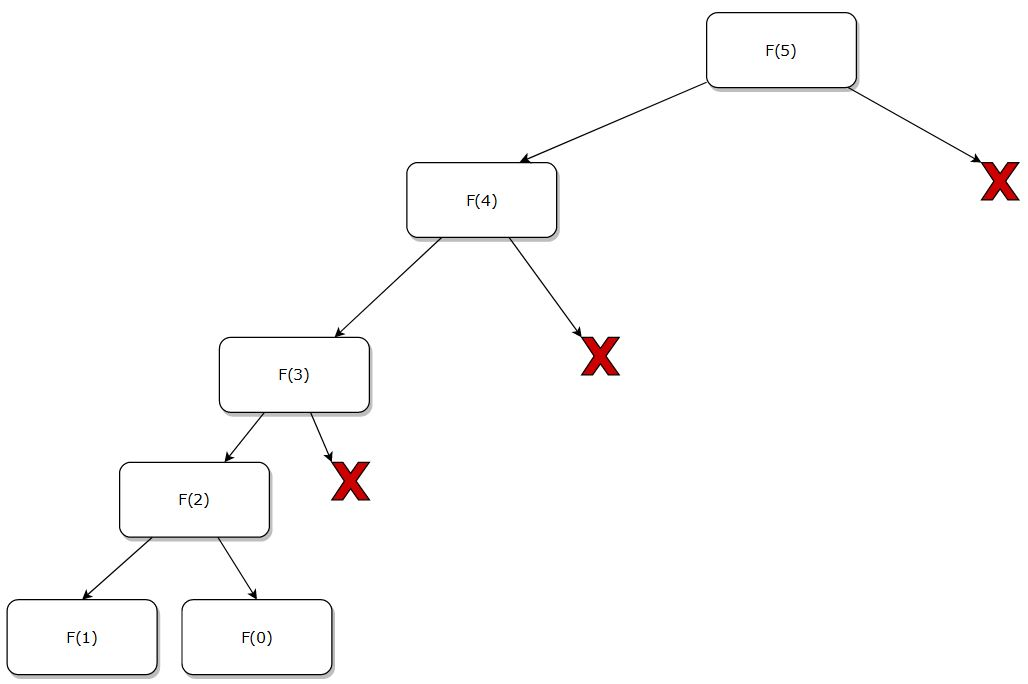
\includegraphics[scale=0.3]{Fibo.JPG}
\end{figure}

\pagebreak

%%%%%%%%%%%%%%%%%%%%%%%%%%%%%%%%%%%%%%%%%%%%%%%%%%%%%%%%%%%%%%%%%%%%%%%%%%%%%%%%%%%%%%%%%%%%%%%%%%%%%%%%%%
\subsubsection{Tabulation (Bottom-Up)}

In the bottom-up dynamic programming approach, reorganize the order in which the subproblems is
solved i.e. compute $F(0)$, then $F(1)$, then $F(2)$, and so on.
\begin{figure} [h!]
    \centering
    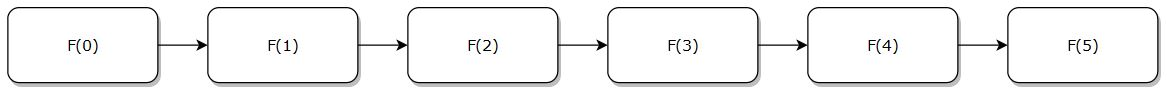
\includegraphics[scale=0.4]{bot.JPG}
\end{figure}

This will allow us to compute the solution to each problem only once, and we’ll only need to save
two intermediate results at a time. \textbf{This will allow us to use less memory space in our code.}

\pagebreak

%%%%%%%%%%%%%%%%%%%%%%%%%%%%%%%%%%%%%%%%%%%%%%%%%%%%%%%%%%%%%%%%%%%%%%%%%%%%%%%%%%%%%%%%%%%%%%%%%%%%%%%%%%
\subsection{Case study: The Rod Cutting Problem}

This case study concerns deciding where to cut a long steel rod into smaller rods for maximum
profit. \par

\textit{Background}: For the inches of the smaller rods to cut into $i$, the price $p_i$ varies.
Determine the maximum revenue $r_n$ obtainable by cutting the rod up and selling the pieces.

\begin{figure} [h!]
    \centering
    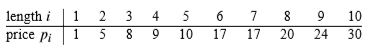
\includegraphics[]{Inche.JPG}
    \caption{Prices for each corresponding inch sold}
\end{figure}

For example, consider the case where the long rod of 4 inches $n=4$ is cut into 4 smaller rods,
there are various ways to cut it as shown:

\begin{figure} [h!]
    \centering
    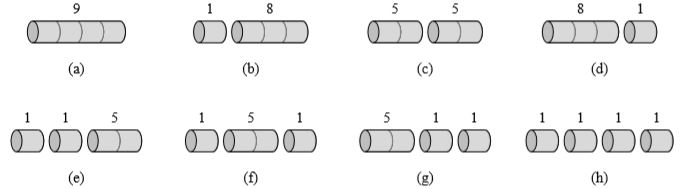
\includegraphics[scale=0.7]{Ways.JPG}
    \caption{Various ways of cutting the rod with the prices shown. Option (c) is clearly the most optimal.}
\end{figure}

Denoting the decomposition into pieces using additive notation: The optimal solution cutting rods
into $k$ pieces for some $1\leq k \leq n$:
$$
    n = i_1 + i_2 + ... + i_k
$$
The rods of length $i_1,i_2,\dots,i_k$ provides sum of corresponding revenue:
$$
    r_n = p_{i_1}+p_{i_2}+\dots+p_{i_k}
$$
Framing the values $r_n$ for $n\geq 1$ in terms of optimal revenue:
$$
    r_n = \text{max}(p_n,r_1+r_{n-1},r_2+r_{n-2},...,r_{n-1}+r_1)
$$
where the first argument $p_n$ corresponds to no cuts at all. \par 

Since it is unknown at the beginning which value of $i$ optimizes revenue, all possible values of
$i$ have to be considered and the one that maximizes revenue chosen.


\pagebreak

%%%%%%%%%%%%%%%%%%%%%%%%%%%%%%%%%%%%%%%%%%%%%%%%%%%%%%%%%%%%%%%%%%%%%%%%%%%%%%%%%%%%%%%%%%%%%%%%%%%%%%%%%%
\subsubsection{Recursive top-down implementation}

\begin{lstlisting}[language = python]
CUT-ROD(p,n):
    if n = 0:
        return 0
    q = -infty

    for i = 1 to n:
        q = max(q.p[i] + CUT-ROD(p,n-1))
    return q
\end{lstlisting}

Points to note:
\begin{itemize}
    \item The procedure takes, as input, an array of $p[1...n]$ of prices and an integer $n$.
    \item Returns the max revenue possible for a rod of length $n$.
    \item If rod is length $n=0$ then no revenue is possible.
    \item Else, initialize the for loop that computes:
    $$
        q=\text{max}_{1\leq i \leq n}(p_1 + \text{CUT-ROD}(p,n-1))
    $$
\end{itemize}

This program is inefficient as the program calls itself recursively with the same parameter values -
solving the same sub-problems repeatedly. \par 

A recursion tree can be created to visualise the number of calls made to CUT-ROD where each node
gives the size $n$ or corresponding sub-problem.

\begin{figure} [h]
    \centering
    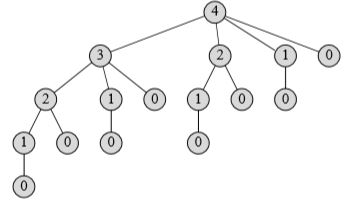
\includegraphics[]{Recursion_tree.JPG}
    \caption{Graphical representaion of the number of calls made to CUT-ROD.}
\end{figure}

Note the exponential behaviour as $n$ increases.

\pagebreak

%%%%%%%%%%%%%%%%%%%%%%%%%%%%%%%%%%%%%%%%%%%%%%%%%%%%%%%%%%%%%%%%%%%%%%%%%%%%%%%%%%%%%%%%%%%%%%%%%%%%%%%%%%
\subsubsection{Using dynamic programming}

As mentioned previous with the two methods: \textbf{bottom-up method} and \textbf{top-down method},
both have the same running time usually with exceptions. The botton-up approach does have better
constant factors since it has less overheads for procedure calls. \par 

\textbf{Top-down with memoization method}:
\begin{lstlisting}
MEMOIZED-CUT-ROD(p,n):
    let r[0...n] be a new array

    for i = 0 to n:
        r[i] = -infty 
    
    MEMOIZED-CUT-ROAD-AUX(p,n,r)

MEMOIZED-CUT-ROD-AUX(p,n,r):
    if r[n] >= 0:
        return r[n]
    if n == 0:
        q=0
    else q = -infty:
        for i = 1 to n:
            q = max(q, p[i] + MEMOIZED-CUT-ROD-AUX(p, n-i, r))
    r[n] = q

    return q
\end{lstlisting}

Points to note:
\begin{itemize}
    \item Main procedure MEMOIZED-CUT-ROD initializes a new auxillary array $r[0...n]$ with value
    $-\infty$ (denotes unknown - \textbf{known values are always positive}). 
    \item Calls helper routine MEMOIZED-CUT-ROD-AUX
    \item Help routine checks to see where desired value is known already (positive or not), if so
    then return the value.
    \item If not, compute the desired value, store it and return it.
\end{itemize}

\pagebreak

\textbf{Bottom-up method}:
Natural ordering of sub-problems: smallest sub-problem solved first.
\begin{lstlisting}
r[0] = 0; // Arrayr[0...n] stores the computed 
            // optimal values
for j = 1 to n do // Consider problems in increasing 
                    // order of size
    q = -infty; 
    for i = 1 to j do // To solve a problem of size j, 
                        // consider all decompositions 
                        // into i and j-i 
        q = max(q, p[i] + r[j-i]);
    end 
    r[j] = q;
end 
return r[n];
\end{lstlisting}

Points to note:
\begin{itemize}
    \item New array created to store the values.
    \item $r[0]$ initialized to 0 since rod length $0$ earns no revenue.
    \item Solve each sub-problem of size $j$ for $j = 1,2,\dots,n$ in order of increasing size.
    \item Direct references to array used instead of making recursive calls to solve the problem.
    \item Return value is the optimal value $r_n$
\end{itemize}

\textbf{Bottom-up method with reconstruction}:
\begin{lstlisting}
// Arrays[0...n] stores the optimal size of the first piece to cut off
r[0] = 0; // Array r[0...n] stores the computed 
          // optimal values
for j = 1 to n do 
    q=-infty;
    for i = 1 to j do // Solve problem of size j
        if q < p[i] + r[j-i] then 
            q = p[i] + r[j-i];
            s[j] = i; // Store the size of the 
                      // first piece
        end 
    end 
    r[j] = q;
end
while n > 0 do // Print sizes of pieces
    Prints[n];
    n=n-s[n];
end
\end{lstlisting}

\pagebreak

%%%%%%%%%%%%%%%%%%%%%%%%%%%%%%%%%%%%%%%%%%%%%%%%%%%%%%%%%%%%%%%%%%%%%%%%%%%%%%%%%%%%%%%%%%%%%%%%%%%%%%%%%%
\section{Greedy algorithms}

Optimization algorithms usually have a sequence of steps with a set of choices at each step. Using
dynamic programming for many problems is sometimes an overkill. A simpler, more efficient algorithm
will work better sometimes i.e. a $O(2^n)$ problem using dynamic programming is $O(n^2)$ but with
greedy algorithms is $O(n)$. \par 

\begin{tcolorbox}[breakable,colback=white]
\textbf{Greedy algorithms}: Any algorithm that follows the problem-solving heuristic of making the locally optimal choice at each stage.
\end{tcolorbox}

Greedy algorithms always make a best possible choice in the hopes that each local optimal solution will
lead to a global optimal solution. Greedy algorithms are not always possible but are faster when
applied. The differences between Greedy Algorithms and Dynamic Programming are summarised below:
\begin{multicols}{2}
    Dynamic Programming:
    \begin{itemize}
        \item Optimization problems
        \item Series of choices
        \item Considers all choices to find which is the best
    \end{itemize}
    
    Greedy Algorithm:
    \begin{itemize}
        \item Optimization problems
        \item Series of choices
        \item Makes the best choice without looking at alternatives
    \end{itemize}
\end{multicols}

%%%%%%%%%%%%%%%%%%%%%%%%%%%%%%%%%%%%%%%%%%%%%%%%%%%%%%%%%%%%%%%%%%%%%%%%%%%%%%%%%%%%%%%%%%%%%%%%%%%%%%%%%%
\subsection{Case study: Activity-selection problem}

The problem of scheduling several competing activities that require exclusive use of a common
resource i.e. classroom that can serve only one activity at a time. \par 

The problem is summarized into the following points:
\begin{itemize}
    \item Let $S={1,2,...,n}$ be the set of activities that compete for the common resource.
    \item Each activity $i$ has a starting time $s_i$ and finish time $f_i$ with $s_i\leq f_i$.
    \item No activities can share the same resource at any time - Activities $i$ and $j$ are
    \textbf{compatible}.
    \item Problem: Select largest set of \textbf{mutually compatible activities}.
\end{itemize}

\pagebreak

\begin{figure} [h!]
    \centering
    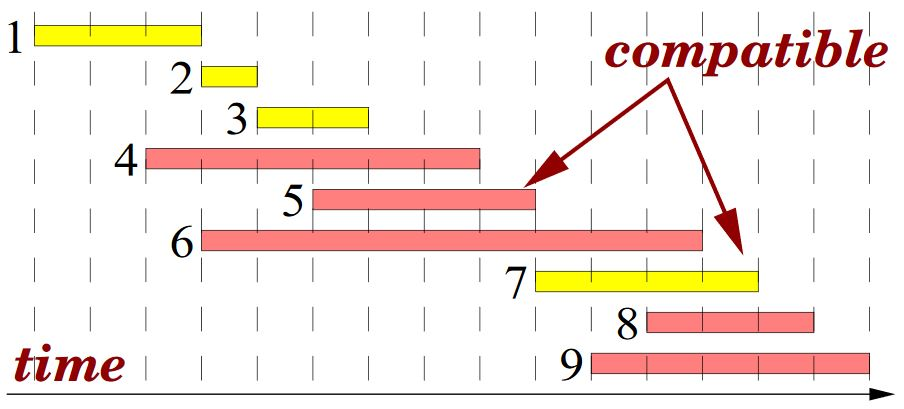
\includegraphics[scale=0.3]{compatible.JPG}
    \caption{Activity 5 and 7 showing compatibility}
\end{figure}

The set of data is then sorted in increasing order of smallest to largest finishing time. After
sorting, it is easy to identify the subsets of mutually compatible activities.
\begin{figure} [h!]
    \centering
    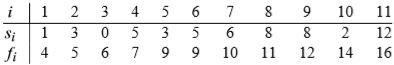
\includegraphics[scale=0.8]{Table.JPG}
    \caption{Table of activities with its start and finishing times}
\end{figure}

The goal is to develop a recursive greedy algorithm. There are several steps involved that result
in the algorithm. \par 

\textbf{Optimal substructure of the activity selection problem}:








%%%%%%%%%%%%%%%%%%%%%%%%%%%%%%%%%%%%%%%%%%%%%%%%%%%%%%%%%%%%%%%%%%%%%%%%%%%%%%%%%%%%%%%%%%%%%%%%%%%%%%%%%%
\subsection{Elements of the greedy strategy}

The general process to develop a greedy algorithm:
\begin{enumerate}
    \item Identify optimal substructure.
    \item Case problem as a greedy algorithm with the greedy choice property.
    \item Write a simple iterative algorithm.
\end{enumerate}

In order to know when a greedy algorithm will solve a particular optimization problem, the
greedy-choice property and optimal substructure is needed. If these two properties can be proved, it
is possible to develop a greedy algorithm.

\pagebreak

%%%%%%%%%%%%%%%%%%%%%%%%%%%%%%%%%%%%%%%%%%%%%%%%%%%%%%%%%%%%%%%%%%%%%%%%%%%%%%%%%%%%%%%%%%%%%%%%%%%%%%%%%%
\subsubsection{Greedy-choice property}

\begin{tcolorbox}[breakable,colback=white]
\textbf{Greedy-choice property}: There exists an optimal solution that is consistent with the greedy
choice made in the first step of the algorithm.
\end{tcolorbox}

This aspect is where greedy algorithms differ from dynamic programming. In dynamic programming, the
choice made at each step depends on solutions of the sub-problems (thus bottom-up manner). In greedy
algorithms, a choice is made depending on the choices made so far, not any future choices. This
means that greedy choice algorithms solves problems in the \textbf{top-down manner}. Proof is
required to show that the greedy choice is always part of the the optimal solution.

%%%%%%%%%%%%%%%%%%%%%%%%%%%%%%%%%%%%%%%%%%%%%%%%%%%%%%%%%%%%%%%%%%%%%%%%%%%%%%%%%%%%%%%%%%%%%%%%%%%%%%%%%%
\subsubsection{Optimal substructure}

Problem shows optimal substructure if an optimal solution to the problem contains within it the
optimal solutions to sub-problems. This property is required by dynamic programming and greedy
algorithms. \par 

%%%%%%%%%%%%%%%%%%%%%%%%%%%%%%%%%%%%%%%%%%%%%%%%%%%%%%%%%%%%%%%%%%%%%%%%%%%%%%%%%%%%%%%%%%%%%%%%%%%%%%%%%%
\end{document}